\Needspace{20\baselineskip}
\section{线程束调度、占用率与指令定位}
\label{l14:sec:scheduling}

\subsection{资源预算如何限制占用率}

\term{占用率}{occupancy}描述一个 SM 中驻留线程束数相对于硬件最大线程束数的比例。\term{理论占用率}{theoretical occupancy}由内核资源需求和启动配置限制，\term{实际占用率}{achieved occupancy}则由执行过程中测得的平均驻留情况得到。驻留表示线程束已经占有相应执行状态，并不要求它当前已经就绪。

设每个线程块有 $T_b$ 个线程，对应 $w_b=\lceil T_b/32\rceil$ 个线程束；一个 SM 允许的最大线程数、线程束数和线程块数分别为 $T_{\max}$、$W_{\max}$、$B_{\max}$。设寄存器容量为 $R_{\mathrm{SM}}$，共享内存容量为 $S_{\mathrm{SM}}$，每块实际占用量为 $R_b$ 和 $S_b$，包含需要计入的驱动保留与分配取整。在简化资源预算中，可驻留线程块数 $B_{\mathrm{res}}$ 满足
\begin{equation}
 B_{\mathrm{res}}\leq\min\left\{
 B_{\max},\left\lfloor\frac{T_{\max}}{T_b}\right\rfloor,
 \left\lfloor\frac{W_{\max}}{w_b}\right\rfloor,
 \left\lfloor\frac{R_{\mathrm{SM}}}{R_b}\right\rfloor,
 \left\lfloor\frac{S_{\mathrm{SM}}}{S_b}\right\rfloor
 \right\},\qquad
 O_{\mathrm{theory}}=\frac{B_{\mathrm{res}}w_b}{W_{\max}}.
 \label{l14:eq:occupancy}
\end{equation}
当实际分配量 $S_b=0$ 时，应略去共享内存这一限制项。寄存器需求不能总是直接用每线程寄存器数乘线程数，因为真实分配会按线程束、线程块或子分区等硬件粒度取整；更详细的资源限制还要由目标设备的占用率报告确认。

考虑一个明确的预算例子：每个 SM 最多驻留 $1536$ 个线程、$48$ 个线程束和 $16$ 个线程块，具有 $65536$ 个 $32$ 位寄存器及 $100$ KiB 可用共享内存。内核每块 $256$ 个线程，即 $8$ 个线程束；每线程需要 $32$ 个寄存器，共享内存预算中的每块总占用量为 $16$ KiB。暂时忽略寄存器的额外分配取整，则每块占 $8192$ 个寄存器，五个限制依次为 $16,6,6,8,6$，最多可驻留 $6$ 块，对应 $48$ 个线程束和 $100\%$ 理论占用率。

若只把寄存器用量提高到每线程 $64$ 个，每块需要 $16384$ 个寄存器，寄存器上限就变成 $4$ 块，于是最多驻留 $32$ 个线程束，占用率降至 $32/48\approx66.7\%$。这并不能单独判断粗化后的内核是否更慢：新增寄存器也可能减少重复读取、保存更多独立累加器，从而改善每个线程束的执行效率。这个预算例子中的硬件数量用于演示计算，不作为所有 GPU 的通用规格。

实际运行还受工作量分布影响。线程块太少、不同块执行时间不一致，以及最后一轮只剩少量工作，都可能使实际占用率低于理论值。若每轮能容纳 $B_{\mathrm{res}}N_{\mathrm{SM}}$ 个线程块，但总块数不能被该数量整除，末轮便无法像满负载阶段那样填满设备。报告中的各项平均值还可能使用不同的活跃周期口径，因此需要同时检查 SM 活动和整个时间线。即使线程束槽位已占满，边界线程束中的部分线程也可能没有有效输出。

例如，若设备同时能容纳 $264$ 个线程块，总工作量原本包含 $1584$ 块，则可以形成 $6$ 轮满负载执行。若粗化后块数变为 $396$，就形成一轮完整工作和一轮只有 $132$ 块的尾部工作。假定各块耗时相同、分配理想，按两个完整轮次的容量计算，槽位利用比例仅为 $396/(2\times264)=75\%$。这个比例描述网格规模与驻留容量不匹配带来的尾部损失；粗化还会改变每块耗时和资源需求，因此它不能直接预测最终加速比。

\subsection{从驻留到就绪，再到实际发射}

线程束调度器维护一组驻留线程束。每周期先检查哪些线程束的下一条指令已具备执行条件，再从这些就绪线程束中选择可发射者。因此，调度报告中的\term{驻留线程束}{active warps}、\term{就绪线程束}{eligible warps}和\term{已发射线程束}{issued warps}分别对应候选集合、当前具备条件的子集和实际发射行为。

图\ref{l14:fig:scheduler}给出的例子中，每调度器的理论上限为 $12$ 个线程束，平均实际驻留 $11.61$ 个，平均就绪却只有 $0.75$ 个，平均每周期发射约 $0.46$ 个线程束。没有就绪线程束的周期约占 $53.89\%$。驻留状态已经接近满额，主要问题是很多线程束同时在等待，调度器缺少可以立即发射的工作。

\begin{figure}[htbp]
\centering
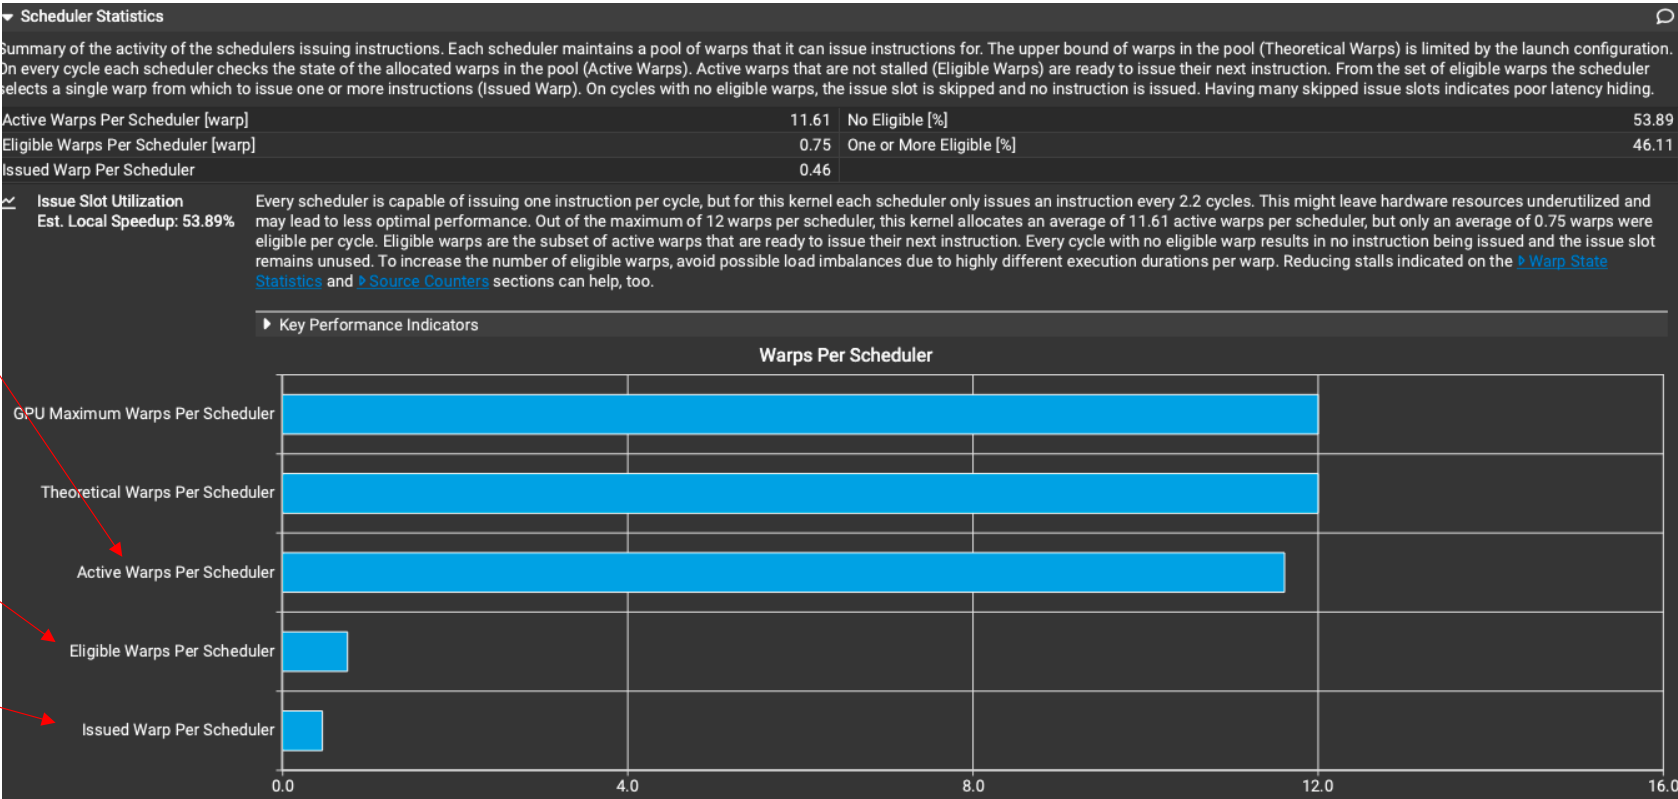
\includegraphics[width=\textwidth]{scheduler.png}
\caption{每调度器的理论、驻留、就绪和发射线程束统计。平均驻留数量接近上限，而就绪与发射数量明显较低，说明需要进一步检查等待原因。}
\label{l14:fig:scheduler}
\end{figure}

平均每周期发射 $0.46$ 个线程束，可理解为调度器平均约每 $1/0.46\approx2.17$ 周期发射一次。报告中的“每条发射指令对应的线程束周期”还会把各驻留线程束经历的周期汇总，示例值约为 $25.18$，其中包含被选中、就绪但未被选中以及停顿等状态。两者的分母不同：前者看调度器整体的发射节奏，后者反映每次指令发射所对应的线程束周期。粗略地，$11.61/0.46\approx25.2$，可以帮助理解两个数字为何处于不同数量级。

如果驻留数量很低，应先检查线程块规模、寄存器、共享内存和网格大小；如果驻留充足而就绪很少，就应检查数据依赖、存储等待与同步；如果就绪线程束较多而目标流水线已经持续忙碌，则要考虑其接收能力和指令组合。这一顺序能把占用率与真正的发射瓶颈联系起来。
